\documentclass{standalone}
\usepackage{tikz}
\begin{document}
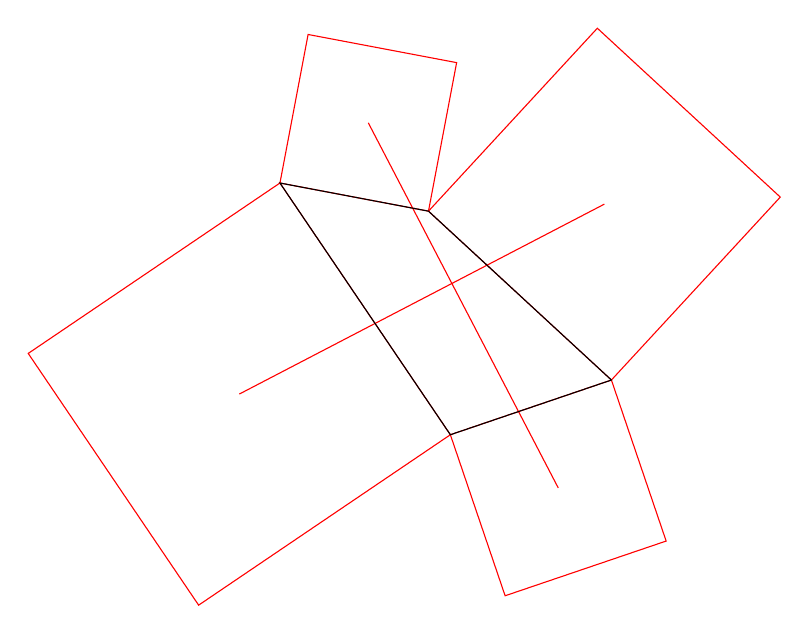
\begin{tikzpicture}[x=1pt,y=1pt]
\draw[red] (158.25,-85.79) -- (224.35,-146.81) -- (285.37,-80.71) -- (219.27,-19.69) -- cycle;
\draw[red] (104.58,-75.62) -- (158.25,-85.79) -- (168.42,-32.12) -- (114.75,-21.95) -- cycle;
\draw[red] (166.16,-166.58) -- (104.58,-75.62) -- (13.62,-137.20) -- (75.20,-228.16) -- cycle;
\draw[red] (244.13,-205.00) -- (224.35,-146.81) -- (166.16,-166.58) -- (185.94,-224.77) -- cycle;
\draw[red] (89.89,-151.89) -- (221.81,-83.25);
\draw[red] (136.50,-53.87) -- (205.14,-185.79);
\draw (104.58,-75.62) -- (166.16,-166.58) -- (224.35,-146.81) -- (158.25,-85.79) -- cycle;
\end{tikzpicture}
\end{document}
